\documentclass{article}
\usepackage{graphicx} % Required for inserting images
\usepackage{amsmath}
\usepackage{amssymb}
\usepackage{booktabs}
\usepackage{caption}
\usepackage{float}
\usepackage[backend=biber, style=ieee]{biblatex}
\addbibresource{references.bib}
\usepackage{subcaption}
\usepackage{placeins}

\usepackage{tikz}
\usetikzlibrary{shapes,arrows,positioning}           % for architecture diagram
\usepackage{booktabs}                                 % for tables
\usepackage{pgfplots}                                % for plots
\pgfplotsset{compat=1.17}
\usepackage{graphicx}

\usepackage{tikz}
\usetikzlibrary{shapes,arrows,positioning}
\usepackage{booktabs}
\usepackage{pgfplots}

\setlength{\parindent}{0pt}
\setlength{\parskip}{\baselineskip}

\title{Lab 3.2 - FMRI, Stat 214, Spring 2025\vspace{-2em}}
\date{April 2025}

\begin{document}

\maketitle

\section{Introduction}

Mapping how the brain processes language can produce insights into comprehension and emotion. In this project, we analyze fMRI data from experiments conducted by Alexander Huth and his team at UT Austin to predict brain activity using natural language processing. Specifically, we extract meaningful embeddings from podcast transcriptions using NLP and use these embeddings to predict fMRI voxel responses. We are provided with a set of podcast transcriptions along with fMRI data from two subject-story pairs, where each row represents the fMRI measurement and the features are the voxel readings. We also have the raw text for each story, which we’ll use to generate embeddings that help predict these responses.

We generated embeddings using four methods: bag-of-words, Word2Vec, GloVe, and with a BERT-style transformer, to improve our prediction models. For Word2Vec and GloVe, we used pre-trained models sourced online: Word2Vec was trained on the Google News dataset and GloVe was trained on a Twitter dataset containing 2 billion tweets, 27 billion tokens, and a vocabulary of 1.2 million words. Our BERT-style tranformer was trained on our training dataset of 89 stories and validated using our validation set for hyperparameter tuning. We then used these embeddings as inputs to train and evaluate our linear models.

\section{Embeddings}

Before extracting embeddings, we randomly split the stories into training and test sets, allocating 80\% to training and 20\% to testing, so that we could fit and evaluate our models per subject. We chose a random split because there was no clear chronological pattern or similarity between the stories that would justify a structured partition. 

\subsection{Bag-of-Words}

Our first method to generate embeddings was bag-of-words. 
This method represents each story as a vector that counts how often each word appears, ignoring word order and contextual meaning but capturing overall word frequency. Essentially, each story is converted into a vector of counts based on the full vocabulary built from all training stories. Each position in the vector represents a word from the full vocabulary, and the value at that position is the number of times that word appears in the specific story. Frequency might be important because it highlights which words are most prominent in a text, which may correlate with key themes that influence brain activity. It also servers as a baseline for other, more complex methods like Word2Vec and GloVe. 

After this step, our feature set (story embeddings) had a different number of rows than our fMRI response data, causing a dimensional mismatch. To address this, we downsampled the embeddings and trimmed the first 5 and last 10 seconds to align the dimensions.

Lastly, we created lagged versions of our features with delays ranging from 1 to 4 seconds using the make delayed function. This function generates lagged versions of the input features to incorporate temporal context into our model's predictors. The function takes our input array, where rows represent time points and columns represent features, and a list of delay values, [1, 2, 3, 4] in our case. For each delay value, the function created a new matrix with shifted data based on the specified delay. If the shift resulted in missing data at the top of our matrix, then these spots were filled with zeros. The function then concatenates all of these delayed matrices horizontally so that our result is a new matrix with lagged features.

\subsection{Word2Vec}

Our next method was Word2Vec, using a pre-trained model sourced online, trained on the Google News dataset, which contains 300-dimensional vectors for 3 million words and phrases.

Word2Vec is a predictive model that uses a shallow neural network to learn word embeddings by focusing on the immediate context of words. It does this through a sliding window over the text and predicting a word from its surrounding context (or vice versa), using various methods like 'skip-gram' or 'continuous bag-of-words'. 

Unlike Bag-of-Words, Word2Vec captures contextual relationships by positioning words with similar contexts closer together in the embedding space. It learns vector representations based on nearby words in the text, enabling it to encode semantic patterns, such as word similarities, for a more nuanced representation that likely improves NLP task performance.

\subsection{GloVE}

Our third embedding method was GloVe, using a pre-trained model sourced online, trained on a Twitter dataset containing 2 billion tweets, 27 billion tokens, and a vocabulary of 1.2 million words.

GloVe is a count-based method that computes a co-occurrence matrix for the dataset and factorizes it to learn word vectors. It uses ratios of co-occurrence probabilities to position words with similar contexts closer together in the embedding space. This produces vector representations that reflect broad patterns of word usage, which creates a more nuanced representation than bag-of-words and can thus improve NLP task performance.

\subsection{BERT-style transformer}


Our final embedding generation method was a BERT-style transformer. BERT uses a transformer architecture with self-attention mechanisms to generate embeddings that capture the meaning of a word based on its surrounding context, unlike Word2Vec and GloVe, which rely on local context or co-occurrence statistics. This allows BERT to produce more nuanced, context-sensitive representations, which can improve performance in NLP tasks by better reflecting the semantic and syntactic roles of words in a story. After training, we extracted embeddings for each story in our dataset using the trained encoder.


\subsubsection{Model Architecture}

The encoder comprises an embedding layer, $N$ stacked transformer blocks, a final layer norm, and an output head for masked language modeling (MLM) predictions. Input text is first tokenized with the “BERT-Base, Uncased” tokenizer from HuggingFace, producing input IDs, token-type IDs, and attention masks. Each transformer block implements multi-head self-attention followed by a two-layer feed-forward network. Figure~\ref{fig:encoder-layer} visualizes one encoder layer. Arrows indicate data flow between submodules.

\begin{figure}[ht]
  \centering
  \resizebox{\textwidth}{!}{%
    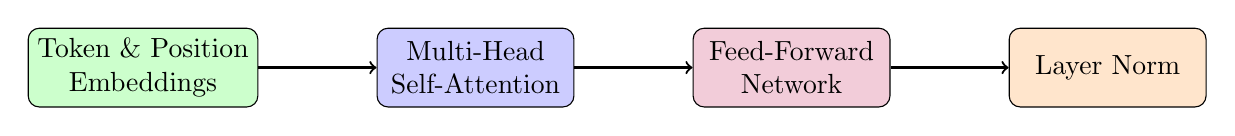
\begin{tikzpicture}[
        block/.style = {rectangle, draw, rounded corners, minimum height=1cm, minimum width=2.5cm, align=center},
        arrow/.style = {->, thick},
        embed/.style = {block, fill=green!20},
        attn/.style  = {block, fill=blue!20},
        ffn/.style   = {block, fill=purple!20},
        norm/.style  = {block, fill=orange!20}
      ]
      \node[embed] (emb) {Token \& Position\\Embeddings};
      \node[attn, right=1.5cm of emb] (attn) {Multi-Head\\Self-Attention};
      \node[ffn,  right=1.5cm of attn] (ffn) {Feed-Forward\\Network};
      \node[norm, right=1.5cm of ffn] (norm){Layer Norm};

      \draw[arrow] (emb) -- (attn);
      \draw[arrow] (attn) -- (ffn);
      \draw[arrow] (ffn) -- (norm);
    \end{tikzpicture}%
  }
  \caption{One layer of the bidirectional transformer encoder.}
  \label{fig:encoder-layer}
\end{figure}


\subsubsection{Hyperparameters}

\begin{table}[h]
  \centering
  \begin{tabular}{ll}
    \toprule
    \textbf{Parameter}                & \textbf{Value}       \\
    \midrule
    Epochs                            & 200                  \\
    Batch size                        & 32                   \\
    Learning rate                     & $1\times10^{-4}$     \\
    MLM probability                   & 15\%                 \\
    Maximum sequence length           & 256                  \\
    Hidden size   & 128                  \\
    Number of heads                   & 2                    \\
    Number of layers           & 2                    \\
    Intermediate size  & 256                  \\
    \bottomrule
  \end{tabular}
  \caption{Hyperparameter values selected for the final model}
  \label{tab:user-hyperparams}
\end{table}


Table~\ref{tab:user-hyperparams} lists the hyperparameters used in our BERT‐style encoder. Below we provide a brief description of each:

\begin{description}
  \item[Epochs]  
    Number of complete passes over the training corpus.  More epochs allow the model to learn more thoroughly but risk over‐fitting as we can see in Figure $\ref{fig:loss}$

  \item[Batch size]  
    Number of training examples processed simultaneously before updating model weights.  

  \item[Learning rate ($1\times10^{-4}$)]  
    Step size used by the optimizer (AdamW) for weight updates.  
    A higher learning rate can accelerate convergence but may cause instability and also overfitting (see the hyperparameters selection discussion).

  \item[MLM probability]  
    Fraction of input tokens randomly masked at each training step.  The model learns to predict these masked tokens from context. $15 \%$ is a standard value.

  \item[Maximum sequence length]  
    Maximum number of tokens per input sequence.  
    Sequences shorter than this length are padded, while longer ones are truncated.  

  \item[Hidden size]  
    Dimensionality of token embeddings and transformer outputs.  Higher values increase representational power at the cost of more parameters.

  \item[Number of heads]  
    Number of parallel attention mechanisms in each self‐attention layer. More heads allow attending to diverse features.

  \item[Number of layers ]  
    Depth of the encoder (number of stacked transformer blocks).  

  \item[Intermediate size ]  
    Dimensionality of the inner feed‐forward network in each transformer block.  
    Typically set to 2–4 times the hidden size in the litterature.  
\end{description}


\subsubsection{Training and selection of the BERT Encoder model hyperparameters}

We employed cross‐validation both to evaluate generalization and to guide hyperparameter tuning. Our 101-text corpus was randomly split into 82 training and 19 test examples. We trained the encoder using a masked-language-modeling objective. After first identifying an appropriate learning rate, we concentrated on tuning the number of attention heads and transformer layers, with results shown in Figure \ref{fig:loss}. Next, we adjusted the hidden-state and intermediate-layer dimensions, and finally we explored several regularization strategies (such as dropout and AdamW weight decay) to mitigate overfitting on our  small dataset.

\begin{figure}[H]
  \centering
  \includegraphics[width=0.8\textwidth]{train_loss.png}
  \includegraphics[width=0.8\textwidth]{val_loss.png}
  \caption{(\textbf{Top}) Training loss for different number of heads and layers . (\textbf{Bottom}) Corresponding validation loss curves, highlighting overfitting in larger models.}
  \label{fig:loss}
\end{figure}

All configurations experience a steep reduction in training loss early in training.  However, only the smallest models maintains a stable validation loss.  The largest one exhibit a pronounced divergence between training and validation curves after a few hundred steps—clear evidence of overfitting on our limited dataset. \\

Despite attempts at regularization (e.g.\ AdamW weight decay and dropout), the fundamental constraint is the small data volume, which limits the efficacy of such techniques.  Consequently, we select the smallest and therefore most parcimonious model as our final architecture, as it provides the best trade‐off between representational capacity and generalization. \\


To further refine the model, we performed a logarithmic grid search over three key parameters:  
\textbf{Hidden size : } $d_{\mathrm{model}}\in\{64,128,256,512\}$ ; \textbf{Intermediate size }$d_{\mathrm{ff}}\in\{256,512,1024,2048\}$ and \textbf{MLM probability : }$p_{\mathrm{mlm}}\in\{0.10,0.15,0.20\}.$



Each combination was evaluated on the validation set for its MLM prediction loss.  The optimal configuration was found to be
\[
\bigl(d_{\mathrm{model}},\,p_{\mathrm{mlm}},\,d_{\mathrm{ff}}\bigr)
=\bigl(128,\;0.15,\;256\bigr),
\]
which achieved the lowest validation error. The selected intermediate size \(d_{\mathrm{ff}}=256\) is twice the hidden size \(d_{\mathrm{model}}=128\), in line with standard Transformer design guidelines that recommend \(d_{\mathrm{ff}}=2\times d_{\mathrm{model}}\) (or up to \(4\times\)), thereby confirming the stability and plausibility of our chosen hyperparameters. To avoid overcrowding the main text, all training logs, hyperparameter configurations, and supplementary results are publicly available on Weights \& Biases at:
\noindent\url{https://wandb.ai/ibrahim_anagaa-university-of-california-berkeley/bert-mlm?nw=nwuseribrahim_anagaa}
This transparent presentation of our experiments enhances both reproducibility and trustworthiness.


A final important point is that the true objective of this lab is not the development of a BERT encoder itself, but rather the prediction of fMRI voxel intensities from stories heard by some subjects. The masked‐language‐modeling embeddings described above serve only as a first‐stage feature extractor. Thus, most of our experimental effort should be devoted to optimizing the downstream regression models that map these embeddings to neural responses, rather than further refining the encoder.

\subsubsection{Outputs of the BERT-style encoder}

To align the embeddings with the fMRI data, we downsampled the embeddings and trimmed the first 5 and last 10 seconds to match the dimensions of the response data, addressing the dimensional mismatch. Finally, we created lagged versions of these embeddings with delays ranging from 1 to 4 seconds using the \texttt{make\_delayed} function, as described in the Bag-of-Words section, to incorporate temporal context into our model's predictors.

\section{Modeling}

\subsection{Fitting the ridge regression}

For each patient, we partition the data into training and testing sets as illustrated in Table \ref{tab:train_test}. We then fit a model for each subject and for each type of embedding used. We opted for this particular split because the goal is to predict voxel intensities for new stories for each subject.\\ 

\begin{table}[h]
\centering
\begin{tabular}{|c|c|c|}
\hline
& \textbf{Training Set} & \textbf{Test Set} \\ \hline
         \textbf{Number of Stories}                  & 82                  & 19                \\ \hline
\end{tabular}
\caption{Train/Test split}
\label{tab:train_test}
\end{table}

In Lab 3.1, we generated Bag-of-Words, Word2Vec, and GloVe embeddings for each story, created their lagged versions, and fitted ridge regression models to predict fMRI responses. The lagged GloVe model performed best based on mean and median correlation coefficients (CC) between predicted voxel intensities and true voxel intensities. In Lab 3.2, we derived embeddings from our trained BERT-style transformer encoder, generated lagged features, and fit a ridge regression model for the same task. The ridge regularization coefficients, \(\alpha\), are determined through a cross-validation scheme described by the following optimization problem:

\[
\min_{\theta \in \mathbb{R}^{D \times V}} \|Y - X\theta\|_2^2 + \alpha^T\|\theta\|_2^2
\]

Where \( \| \theta \|_2^2 \) is vector with coefficient $i$ representing the \(L_2\) norm squared of the \(i\)-th column of the matrix \(\theta\), calculated as follows:

\[
(\| \theta \|_2^2)_i = \sum_{j=1}^D \theta_{j,i}^2
\]

To optimally tune the vector \(\alpha\), we employ a five-fold cross-validation approach, dividing the stories into 5 equal parts. The selection of \(\alpha\) was based on maximizing the mean correlation coefficient across the validation folds.

\subsection{Evaluation of the BERT-style transformer}

The results for subject 2 are summarized in Table 3. Here, we compare our BERT-style encoder with the best performing methods from lab 3.1. Comparison of these two models is also done through our stability analysis, as this displays both model's generalizability.

\begin{table}[H]
  \centering 
  \begin{tabular}{@{}lcccccc@{}} 
    \toprule
    Metric & \textbf{BERT} & \textbf{Lagged BERT} & \textbf{Glove} & \textbf{Lagged Glove} & \textbf{W2V} & \textbf{Lagged W2V} \\
    \midrule
    Mean     & 0.0029 & 0.0043 & 0.0114 & 0.0151 & 0.0119 & 0.0150 \\
    Median   & 0.0023 & 0.0035 & 0.0088 &  0.0117 & 0.0091 & 0.0115 \\
    Top 1\%  & 0.0407 & 0.0471 & 0.0711 & 0.0867 & 0.0739 & 0.0863  \\
    Top 5\%  & 0.0274 & 0.0314 & 0.0487 & 0.0576 & 0.0502 & 0.0571  \\
    \bottomrule
  \end{tabular}
  \caption{\textbf{Performance Comparison for Subject 2.} The Bert-style transformer encoder displays the worst performance among previous models. The Lagged GloVe model achieves the highest mean CC, top 1\%, and top 5\% percentile. Lagged feature matrices generally exhibit better performance in all metrics.}
  \label{tab:model_performance}
\end{table}

We can see from above that our lagged BERT model performed substantially worse, in terms of mean and median CC's, than our other embedding methods, likely due to the lack of data we trained our transformer on. We can also see that our top 1\% and top 5\% performance on our lagged BERT model was worse than our other well performing methods from lab 3.1, hinting that our model was generally worse than the alternatives. 

Further evaluation of the Lagged BERT model performance is conducted by analyzing its distribution (Figure 3) as a comparison to our lagged Glove model. Both distribution's exhibits a pronounced right tail, suggesting that while our models do not perform uniformly across all voxels, they generally tend towards predictions that correlate positively with the true values. Our lagged BERT model had a smaller proportion of values displaying a positive correlation than our lagged Glove model and a thinner right tail, both indicating that our Glove model had better predictive power for this task. 

Broadly, the low absolute correlations for both models reflect very high measurement noise and a largely non-linear mapping between the stimuli and our BOLD responses that a linear ridge regression can't perfectly capture. The specific performance gap between lagged BERT and lagged Glove is likely due to our lack of data. Our BERT-style encoder was trained from scratch on only the handful of podcast transcripts we were supplied with, a number that is several orders of magnitude smaller than the text that the Glove model was trained on. 


\begin{figure}[H]
\centering
\captionsetup{width=\textwidth}
\includegraphics[width=1.05\textwidth]{figs/corr_hist_BERT_vs_GloVe.png}
\captionof{figure}{\textbf{The distribution of the CC for the lagged Glove and BERT embeddings across voxels.}}
\label{fig:dist}
\end{figure}

PCS analysis can also serve as a framework for model comparison. In a PCS analysis, voxel intensity serves as an indicator of the brain's response to language stimuli, but the underlying mechanisms are complex so we should do some stability analyses to accurately measure our results.

\subsection{Stability analysis}

For stability analysis, we examined how the model performs by subject and by story within the test set as shown in table 4 below. For Subject 2, using our BERT-style transformer, it's clear that our model encountered difficulties with a few stories such as \textit{googling strangers and kentucky bluegrass} and \textit{life} which both had negative mean correlation coefficients. With the GloVe-based model, we again saw a few poorly-predicted stories, but none of the mean or median CCs fell below zero. Also, nearly every story’s mean CC under GloVe exceeded its counterpart from the BERT-style encoder, underscoring that the GloVe embeddings provided more predictive power than the embeddings learned by our small, task-specific BERT.

This pattern was also explored for stability with subject 3 in table 5; however, the model's performance on the test stories varied significantly between subjects. This disparity could be interpreted as an indication of the model's instability, which is explained by the inherently noisy nature of fMRI data, lack of training data for our BERT-style transformer, and the complex dynamics between stimuli and cerebral responses. The poor performance of BERT compared to Glove persisted among almost all stories, further indicating that this lack of data was hindering our ability to derive genuine predictive power. 

Overall, the model's performance variability between stories and between subjects suggests instability that can be explained by noisy data, a lack of training data for our BERT-style transformer, and complex dynamics between our predictors and response that cannot be explained through a linear problem. 

\begin{table}[H] 
  \centering
  \caption{Comparison of CC Metrics for validation stories (Subject 2) using BERT embeddings and GloVe embeddings. Stories are sorted by Mean CC.}
  \label{tab:story_cc_metrics_comparison}
  \begin{tabular}{lcccc}
    \hline
    \multicolumn{5}{c}{\textbf{BERT Embeddings}} \\
    \hline
    \textbf{Story Name} & \textbf{Mean CC} & \textbf{Median CC} & \textbf{Top 1\% CC} & \textbf{Top 5\% CC} \\
    \hline
    sweet as pie                  & 0.0153 & 0.0144 & 0.2351 & 0.1665 \\
    the triangle shirtwaist connection & 0.0148 & 0.0127 & 0.2265 & 0.1540 \\
    wild women and dancing queens & 0.0114 & 0.0108 & 0.2030 & 0.1438 \\
    avatar                      & 0.0107 & 0.0106 & 0.1577 & 0.1120 \\
    beneath the mushroom cloud  & 0.0099 & 0.0079 & 0.1802 & 0.1218 \\
    escaping from a dire diagnosis & 0.0061 & 0.0059 & 0.1487 & 0.1062 \\
    the postman always calls    & 0.0058 & 0.0058 & 0.1331 & 0.0937 \\
    under the influence         & 0.0042 & 0.0039 & 0.1595 & 0.1110 \\
    fire test for love          & 0.0031 & 0.0028 & 0.1507 & 0.1071 \\
    Tetris                      & 0.0018 & 0.0016 & 0.1568 & 0.1086 \\
    birth of a nation           & 0.0011 & 0.0009 & 0.1607 & 0.1126 \\
    laws that choke creativity  & 0.0011 & 0.0012 & 0.1291 & 0.0904 \\
    the secret to marriage      & 0.0010 & 0.0011 & 0.1591 & 0.1113 \\
    christmas 1940              & 0.0006 & -0.0001 & 0.1876 & 0.1286 \\
    souls                       & 0.0003 & 0.0003 & 0.1436 & 0.0976 \\
    when mothers bully back     & 0.0001 & 0.0001 & 0.1542 & 0.1076 \\
    a fear stripped bare        & -0.0004 & -0.0012 & 0.1346 & 0.0907 \\
    life                        & -0.0005 & -0.0009 & 0.1343 & 0.0917 \\
    googling strangers and kentucky bluegrass & -0.0028 & -0.0026 & 0.1217 & 0.0844 \\
    \hline
    \multicolumn{5}{c}{\textbf{GloVe Embeddings}} \\
    \hline
    \textbf{Story Name} & \textbf{Mean CC} & \textbf{Median CC} & \textbf{Top 1\% CC} & \textbf{Top 5\% CC} \\
    \hline
    wild women and dancing queens & 0.0278 & 0.0253 & 0.2403 & 0.1706 \\
    sweet as pie                  & 0.0219 & 0.0210 & 0.2530 & 0.1821 \\
    a fear stripped bare           & 0.0211 & 0.0190 & 0.1756 & 0.1234 \\
    when mothers bully back        & 0.0177 & 0.0161 & 0.1888 & 0.1320 \\
    souls                       & 0.0175 & 0.0154 & 0.1895 & 0.1311 \\
    the postman always calls       & 0.0170 & 0.0153 & 0.1593 & 0.1129 \\
    the triangle shirtwaist connection & 0.0150 & 0.0139 & 0.2202 & 0.1514 \\
    beneath the mushroom cloud     & 0.0140 & 0.0111 & 0.1932 & 0.1283 \\
    googling strangers and kentucky bluegrass & 0.0137 & 0.0118 & 0.1654 & 0.1112 \\
    Tetris                      & 0.0135 & 0.0110 & 0.1878 & 0.1284 \\
    fire test for love             & 0.0118 & 0.0113 & 0.1600 & 0.1149 \\
    the secret to marriage         & 0.0117 & 0.0096 & 0.2010 & 0.1371 \\
    avatar                      & 0.0116 & 0.0086 & 0.2050 & 0.1286 \\
    christmas 1940               & 0.0116 & 0.0102 & 0.2155 & 0.1511 \\
    birth of anation              & 0.0090 & 0.0087 & 0.1677 & 0.1198 \\
    under the influence           & 0.0077 & 0.0074 & 0.1640 & 0.1151 \\
    laws that choke creativity     & 0.0068 & 0.0066 & 0.1282 & 0.0906 \\
    escaping from a dire diagnosis  & 0.0044 & 0.0036 & 0.1538 & 0.1083 \\
    life                        & 0.0015 & 0.0006 & 0.1472 & 0.0994 \\
    \hline
  \end{tabular}
\end{table}

\begin{table}[H] 
  \centering
  \caption{Comparison of CC Metrics for validation stories (Subject 3) using BERT embeddings and GloVe embeddings. Stories are sorted by Mean CC.}
  \label{tab:story_cc_metrics_comparison}
  \begin{tabular}{lcccc}
    \hline
    \multicolumn{5}{c}{\textbf{BERT Embeddings}} \\
    \hline
    \textbf{Story Name} & \textbf{Mean CC} & \textbf{Median CC} & \textbf{Top 1\% CC} & \textbf{Top 5\% CC} \\
    \hline
    christmas 1940              & 0.0270 & 0.0238 & 0.2267 & 0.1609 \\
    birth of a nation           & 0.0181 & 0.0166 & 0.1940 & 0.1387 \\
    beneath the mushroom cloud  & 0.0145 & 0.0124 & 0.1863 & 0.1256 \\
    life                        & 0.0133 & 0.0122 & 0.1450 & 0.1037 \\
    wild women and dancing queens & 0.0112 & 0.0110 & 0.2107 & 0.1499 \\
    googling strangers and kentucky bluegrass & 0.0110 & 0.0101 & 0.1477 & 0.1030 \\
    souls                       & 0.0105 & 0.0095 & 0.1566 & 0.1095 \\
    the postman always calls    & 0.0100 & 0.0082 & 0.1570 & 0.1065 \\
    sweet as pie                & 0.0081 & 0.0077 & 0.2261 & 0.1608 \\
    laws that choke creativity  & 0.0081 & 0.0065 & 0.1501 & 0.1032 \\
    avatar                      & 0.0077 & 0.0073 & 0.1515 & 0.1060 \\
    the secret to marriage      & 0.0071 & 0.0070 & 0.1623 & 0.1153 \\
    a fear stripped bare        & 0.0064 & 0.0062 & 0.1394 & 0.0971 \\
    under the influence         & 0.0062 & 0.0065 & 0.1537 & 0.1102 \\
    fire test for love          & 0.0042 & 0.0042 & 0.1480 & 0.1046 \\
    Tetris                      & 0.0034 & 0.0039 & 0.1625 & 0.1150 \\
    when mothers bully back     & -0.0006 & -0.0007 & 0.1498 & 0.1046 \\
    the triangle shirtwaist connection & -0.0007 & -0.0008 & 0.2015 & 0.1386 \\
    escaping from a dire diagnosis & -0.0018 & -0.0017 & 0.1344 & 0.0934 \\
    \hline
    \multicolumn{5}{c}{\textbf{GloVe Embeddings}} \\
    \hline
    \textbf{Story Name} & \textbf{Mean CC} & \textbf{Median CC} & \textbf{Top 1\% CC} & \textbf{Top 5\% CC} \\
    \hline
    sweet as pie                & 0.0480 & 0.0458 & 0.2878 & 0.2125 \\
    christmas 1940              & 0.0359 & 0.0328 & 0.2364 & 0.1750 \\
    birth of a nation           & 0.0349 & 0.0317 & 0.2460 & 0.1760 \\
    beneath the mushroom cloud  & 0.0331 & 0.0282 & 0.2390 & 0.1585 \\
    wild women and dancing queens & 0.0322 & 0.0312 & 0.2409 & 0.1804 \\
    googling strangers and kentucky bluegrass & 0.0261 & 0.0235 & 0.1857 & 0.1303 \\
    a fear stripped bare        & 0.0203 & 0.0186 & 0.1683 & 0.1182 \\
    fire test for love          & 0.0200 & 0.0200 & 0.1664 & 0.1220 \\
    souls                       & 0.0198 & 0.0175 & 0.1877 & 0.1266 \\
    laws that choke creativity  & 0.0195 & 0.0188 & 0.1588 & 0.1156 \\
    life                        & 0.0187 & 0.0177 & 0.1480 & 0.1089 \\
    avatar                      & 0.0180 & 0.0156 & 0.1970 & 0.1362 \\
    under the influence         & 0.0151 & 0.0147 & 0.1593 & 0.1163 \\
    the postman always calls    & 0.0140 & 0.0125 & 0.1571 & 0.1076 \\
    the secret to marriage      & 0.0136 & 0.0119 & 0.1829 & 0.1294 \\
    when mothers bully back     & 0.0106 & 0.0089 & 0.2103 & 0.1352 \\
    Tetris                      & 0.0105 & 0.0089 & 0.1798 & 0.1244 \\
    the triangle shirtwaist connection & 0.0084 & 0.0069 & 0.2235 & 0.1534 \\
    escaping from a dire diagnosis & 0.0073 & 0.0075 & 0.1631 & 0.1163 \\
    \hline
  \end{tabular}
\end{table}

We can also generate a stability analysis through analyzing the distributions between the stories with the best and worst correlation coefficients using our BERT-style transformer and compare it to our similar distribution from lab 3.1. 

Our last report examined the differences in the CC distribution between the stories \textit{Wild Women and Dancing Queens} and \textit{Life} (Figure \ref{story}). The CC distribution for \textit{Wild Women}, the better-performing story, exhibits greater variability compared to the poorer-performing \textit{Life}. This suggests that the model performs more consistently—albeit poorly—on the voxels associated with the \textit{Life} story, whereas it demonstrates more variability in its performance on the \textit{Wild Women} story. \\

For our Bert-style transformer, figure 4 displays a similar effect, that although our best performing story had a better mean correlation coefficient than our worst performing story, it also had greater variability compared to the poorer-performing story. This suggests that the model can achieve high correlations for certain voxels, but it struggles to maintain that performance across all voxels, leading to a wider spread in CC values and again hints at the models instability. 

\begin{figure}[H]
\centering
\captionsetup{width=\textwidth}
\includegraphics[width=1\textwidth]{./figs/story_1.png}
\captionof{figure}{{Distribution of CC with our BERT embeddings for \textit{Sweet as pie} and \textit{Googling strangers and kentucky bluegrass}, the test stories with the best and worst mean CC scores for subject 2.}}
\label{story}
\end{figure}

\begin{figure}[H]
\centering
\captionsetup{width=\textwidth}
\includegraphics[width=1\textwidth]{./figs/story.png}
\captionof{figure}{{Distribution of CC with our Glove embeddings for \textit{Wild Women and Dancing Queens} and \textit{Life}, the test stories with the best and worst mean CC scores for subject 2.}}
\label{story}
\end{figure}

Lastly, we can examine the CC distribution over both subjects with our Glove method and our Bert-style transformer. Figure 6 shows that the distribution for subject 3 is shifted to the right of the blue curve subject 2, with a mean CC is roughly twice as large and the right tail longer. In other words, a larger fraction of voxels in subject 3 achieve positive correlations and the best-predicted voxels reach higher values, indicating that the model generalises better to subject 3 than to subject 2. We also observed this with our Glove embeddings, hinting that subject 3 yielded a more linearly predictable voxel response, in general, compared to subject 2. 

\begin{figure}[H]
\centering
\captionsetup{width=\textwidth}
\includegraphics[width=1\textwidth]{./figs/comparing_both_subjects.png}
\captionof{figure}{\textbf{Subject2 vs. Subject3 test CC for our model using our BERT embeddings}}
\label{subjects}
\end{figure}

\begin{figure}[H]
\centering
\captionsetup{width=\textwidth}
\includegraphics[width=1\textwidth]{./figs/comparing_both_subjects_glove.png}
\captionof{figure}{\textbf{Subject2 vs. Subject3 test CC for our model using Glove embeddings}}
\label{subjects}
\end{figure}

\subsection{Conclusion}

Our goal was to predict fMRI responses by converting our transcripts of raw texts into four kinds of linguistic features, bag-of-words, Word2Vec, GloVe, and a small BERT-style transformer that we trained ourselves, and then fitting ridge-regression models for each voxel. We tuned the encoder’s hyper-parameters with a grid search that balanced model performance against over-fitting risk which we could validate using our validation set. We fixed the learning rate at 10\^-4 and compared four configurations that varied the number of transformer layers and attention heads. Training loss dropped for every setting, but validation loss began to rise once the model exceeded two layers and two heads, a clear sign of overfitting. We therefore adopted the lightest configuration (2 layers, 2 heads, hidden size 128, intermediate size 256) and retained a dropout rate of 0.1 plus AdamW weight-decay regularization. This model delivered the lowest held-out MLM loss while keeping the embedding dimensionality modest, which in turn helped the downstream ridge regression to remain numerically stable.

Our performance metrics showed that models with contextual information performed better than others, with Word2Vec surpassed the bag-of-words baseline and our BERT-style transformer, and Glove having the highest mean and median correlations overall. Our BERT-style transformer captured some predictiveness of voxel response, but because it was pre-trained on only 89 stories, it did not yet match the performance of the large, publicly trained Glove or Word2Vec vectors. Our stability analysis also touched on several metrics that displayed the superiority of our Glove embeddings over our BERT-style transformer.

% \section{Bibliography}
% Include any references you used in your report here.
\appendix
\section{Academic honesty}

\subsection{Statement}

Here we make the truthful statements: We ourselves designed and performed all the data analysis procedures presented in this report. We ourselves wrote all the texts and produced all the figures in this report. We have included and documented all the procedures in the workflow and the results can be fully reproduced. 

We believe that academic honesty is important because it creates a fair environment for others and ourselves, judging us by our true decisions and work ethic, which allows for a more accurate representation of industry and research.

\subsection{LLM Usage}

We used Large Language Models for some visualizations and grammatical help, but the code and report were done entirely by our group members alone. 

% \subsubsection*{Coding}

% \subsubsection*{Writing}


\end{document}